\chapter{三维人体姿态估计算法性能分析}

根据第二章和第三章提出的堆叠沙漏网络结构以及基于几何约束设计的深度回归模块,本章基于Ubuntu系统上进行3D人体姿态识别算法的原理性验证及性能分析。

\section{堆叠沙漏网络结构的检测算法实现}
第二章所述基于堆叠沙漏网络的人体姿态结构的识别算法,在本节中将会详细介绍其实验过程以及对应的结果分析。

\subsection{数据样本}

在进行算法实验之前,需要对数据样本做初步筛选和处理。本次实验采用MPII数据集作为实验对象,将其中约3000张照片的json信息读取出来,根据annntions文件的包围框数据,提取出对应的目标对象。随机选取其中3000个目标对象,为了使得本阶段实验的科学性。将这3000个目标对象分为两组,一组2500作为训练目标,另一组500个作为测试目标。

\subsection{堆叠沙漏网络的训练步骤}

为了探究堆叠沙漏网络的阶数对于识别效率的提升效果,进行如下实验。
本节中介绍其详细的算法实现流程及其细节。

(1)环境的搭建

整个实验是利用了GPU来进行训练,需要在ubuntu操作系统上运行,采用了python3语言以及pytorch深度学习框架。第一步是搭建显卡驱动,CUDA接口以及miniconda环境。第二步是创建一个专属本次算法实现的python虚拟环境,其中需要将python版本设置为3.6.5以上版本,并在虚拟环境中安装numpy,opencv,pytorch,torchvision等相关依赖。第三步,需要将数据集整理好,放入ubuntu系统中的设置好的工程文件。

(2)准备工作

利用opencv将数据集中的图像信息做初步特征信息的提取,设置为numpy格式,方便以后使用。将含有真实信息的annotions标记文件,按照列表的形式,也要提前读取出来。然后对图片进行数据增广,使其转化为tensor的格式,并且在BGR通道顺序改为RGB通道顺序。在设定好学习率为0.0001,批量数为20等超参数后便开始迭代训练。

在完成一次迭代过程后,选取分数最高的前100个与真实值参与损失函数的计算,完成一次迭代过程,继续下一次的迭代流程。

(3)训练实现

第一步需要将annotions文件夹中的标签文件进行处理,因为MPII数据集的标签为json格式,所以要在训练之前将所有的训练图片以及关节点数据按照列表的格式,保存在GPU的内存里。第二步则需要利用scipy对图片进行读取操作,根据标签文件的box位置,将每张图像中的多个人体目标提取出来,而且需要将尺寸设置为256*256。第三步,则根据pytorch框架的设置原则,根据骨干网路为堆叠沙漏网络的思路,还要将图像信息转化为tensor格式,设置好初始参数开始迭代训练。

每一次迭代完成以后,可以得到一个64*64*16的张量数据,根据热力图的原理,我们选取其中亮度最大的一个点,即可判断此关节点的位置就是最有可能出现的预测位置。在计算损失时,需要将得到的真实张量与真实值做比较。

4)实现人体姿态预测

在训练完成后,需要将每个关节点的预测结果中的三个坐标按照列表的形式返回,结合annotions文件的包围框的标签数据。只要是预测结果在包围框以内的关节点,即可判断这是该目标对象的关节点数据。如果预测顺利,所得到的姿态应该是16张64*64的热力图,对热力图中最亮的点进行位置信息提取,就可以得到三位预测坐标。将三维坐标信息的真实数值和预测值,做对应的评价指标的评价。
	
依次将二阶,四阶,八阶,十六阶沙漏网络进行220次迭代训练

\subsection{训练结果分析}

\begin{figure}[h]
	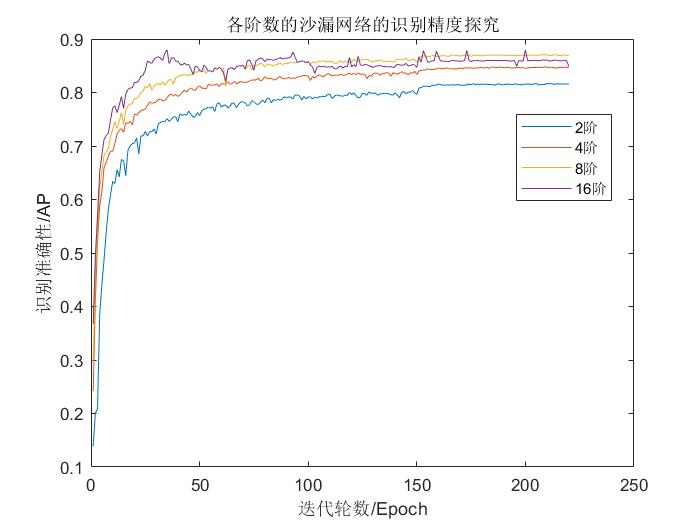
\includegraphics[width=\textwidth]{pic/stacked_hourglass.jpg}
	\caption{各阶堆叠沙漏网络的AP}
	\label{AP_graph}
\end{figure}

结合AP指标来分析,如图\ref{AP_graph}所示

可以得出以下结论:2阶到4阶的堆叠沙漏网络而言,在迭代足够多的情况下,阶数的提升提高了$3.0\%$左右的平均准确率。4阶到8阶的堆叠沙漏网络而言,在迭代足够多的情况下,阶数的提升提高了$1.6\%$左右的平均准确率。8阶到16阶的堆叠沙漏网络而言,初期迭代,识别精度提升很快,在迭代足够多的情况下,阶数的提升反而降低了$0.9\%$的平均准确率。

\begin{figure}[h]
	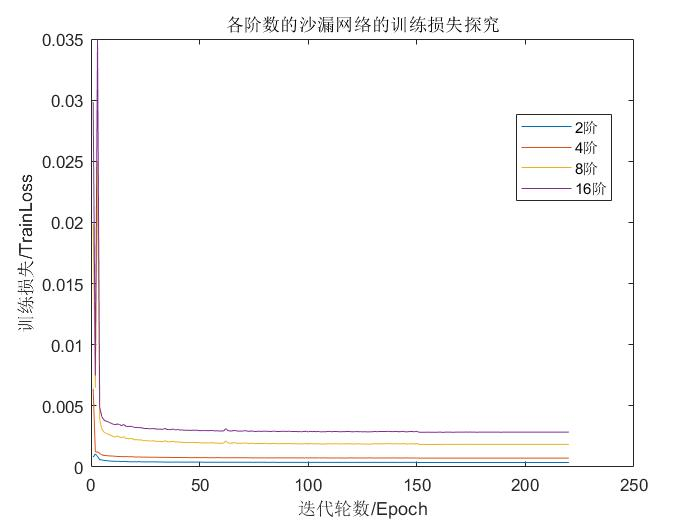
\includegraphics[width=\textwidth]{pic/stacked_hourglass_trainloss.jpg}
	\caption{各阶堆叠沙漏网络的训练误差}
	\label{Loss_graph}
\end{figure}

结合训练误差指标来分析,如图\ref{Loss_graph}所示

可以得到以下结论:训练损失曲线在前四次迭代就迅速下降后趋于平缓,几乎没有发生变化。并且随着堆叠沙漏网络阶数的提升,训练产生的损失反而更大。

总结:随着阶数的提升,确实可以提升识别准确率,但是一旦到达了一定阶数,就不能通过堆叠阶数的方式来提升识别精度,原因一,有可能是阶数过高,有可能在卷积层处理信息时,尽管有残差模块的补助,然而信息流失的概率还是很大,原因二,还有可能是,迭代到后期,在反向传播过程中,由于十六阶的网络复杂度过高,学习率的设置不太合适,导致结果过拟合。

使用MPII数据集标注的方法,结合MPJPE指标来分析。

\begin{table}[]
    \centering
    \begin{tabular}{c|c|c|c|c|c|c|c|c}
        \hline
         阶数 & Head & Shoulder	& Elbow	& Wrist	& Hip & Knee & Ankle & Mean\\
        \hline
         二阶 & 92.16 & 82.63 & 71.55 & 64.31 & 68.74 & 59.00 & 59.07 & 70.84\\
        \hline
         四阶 & 81.56 & 75.35 & 65.23 & 61.29 & 63.58 & 53.64 & 54.51 & 65.02\\
        \hline
         八阶 & 73.59 & 70.09 & 61.49 & 58.94 & 60.39 & 49.35 & 50.23 & 60.58\\
        \hline
         十六阶 & 70.25 & 68.06 & 60.56 & 57.65 & 59.49 & 50.23 & 51.56 & 59.68\\
        \hline
    \end{tabular}
    \caption{各阶堆叠沙漏网络的MPJPE}
    \label{MPII_dataset}
\end{table}

根据试验结果,可以得出以下结论:
2阶到4阶的堆叠沙漏网络而言,在迭代足够多的情况下,阶数的提升提高了5.5mm左右的平均关节误差(MPJPE)。
4阶到8阶的堆叠沙漏网络而言,在迭代足够多的情况下,阶数的提升提高了4.5mm左右的平均关节误差(MPJPE)。
8阶到16阶的堆叠沙漏网络而言,在迭代足够多的情况下,阶数的提升0.9mm的平均关节误差(MPJPE)。

总结:发现阶数的提升,确实能够带来MPJPE指标上的优化,但是到达了一定阶数,提升的效果不太明显。因为阶数越高,训练时间越久,而且效果提升不明显,所以十六阶堆叠沙漏网络的性价比不高。结合工程的实际需要,发现八阶的堆叠沙漏网络是最合适的模型,因此在本文的3D人体姿态估计算法中,最终采用了八阶堆叠沙漏网络。

\section{不同数据集的检测算法和仿真}

因为主流数据集主要有MPII,COCO,HUMAN3.6M,LSP数据集,每种数据集都有不同的标注方法,所以这里探究不同数据集对于人体姿态识别效果优劣的比较。

考虑到HUMAN3.6M的审批获取步骤很麻烦,以及LSP数据集的场景较小,因此这里只对MPII和COCO数据集进行比较。

\subsection{数据样本}

该模型的训练样本为MPII数据集与COCO数据集。其中MPII数据集信息和4.1.1一致,保持不变。对于COCO数据集而言,包含了8601张训练照片和1827张验证照片。经过上一节的分析,最终采用八阶堆叠沙漏网络,对这两个数据集中的训练图片分别进行样本分割。对于MPII训练图片而言,包含了3000个左右的目标样本。为了充分利用训练,本次实验对于MPII数据集而言,使用了2500个目标作为训练样本,500个目标作为验证样本。为了进行对比,对于COCO训练图片而言,本次实验也随机选取了2500个目标对象作为训练样本,500个目标对象作为验证样本。

\subsection{训练步骤}

为了探究不同数据集的标注方法对于识别效率的提升效果,进行如下实验。本节中介绍的算法实现的编译过程,(1)(2)(3)(4)和4.1.2基本类似,这里就不再赘述。

变动如下:(2)而训练网络中的关节点等初始化参数的设置,根据不同数据集的特点分别设置即可。(4)为方便比较不同标注方法,最后按照一个目标对象的所有关节点的位置信息,按照对应标注方法,将其映射回原始图像并且进行关节连线,即可完成人体姿态估计显示任务。

\subsection{训练结果分析}

对MPII,COCO数据集进行训练,得到训练结果如下,结合MPJPE指标来分析

\begin{table}[]
    \centering
    \begin{tabular}{c|c|c|c|c|c|c|c|c}
        \hline
         数据集 & Head & Shoulder	& Elbow	& Wrist	& Hip & Knee & Ankle & Mean\\
        \hline
         MPII & 73.59 & 70.09 & 61.49 & 58.94 & 60.39 & 49.35 & 50.23 & 60.58\\
        \hline
         COCO & 68.35 & 69.35 & 61.39 & 56.25 & 63.29 & 53.35 & 52.96 & 60.72\\
        \hline
    \end{tabular}
    \caption{MPII和COCO数据集的MPJPE}
    \label{com_dataset}
\end{table}

可以得出以下结论:
MPII数据集的标注方法,对于面部特征的标注信息较少,导致面部的几个关节点处理上不如COCO数据集。而COCO数据集,因为对面部信息的标注,使得头部的点标注误差较小。整体比较而言,数据集标注方法的差异,对于标注误差没有很大的影响,可以忽略。

训练结果图示如下:

\begin{figure}[h]
	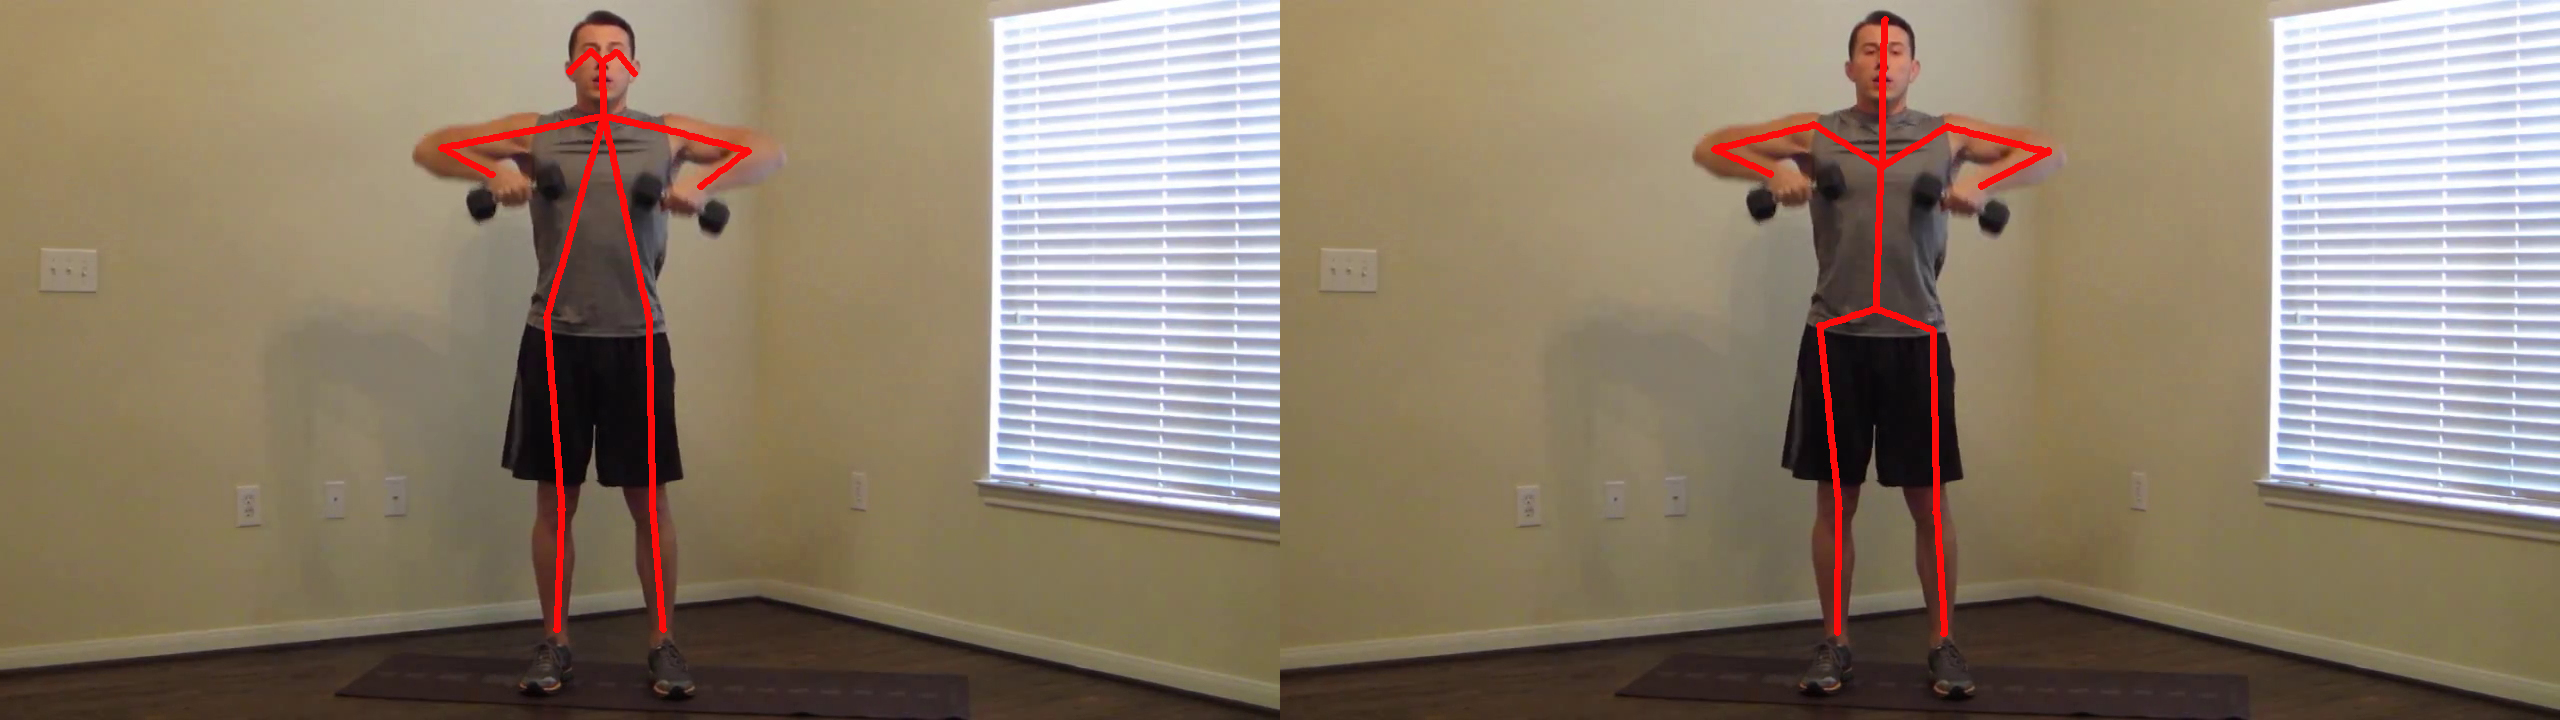
\includegraphics[width=\textwidth]{pic/vs_1.jpg}
	\caption{演示1(左图为COCO标注,右图为MPII标注)}
	\label{vs_1}
\end{figure}

\begin{figure}[h]
	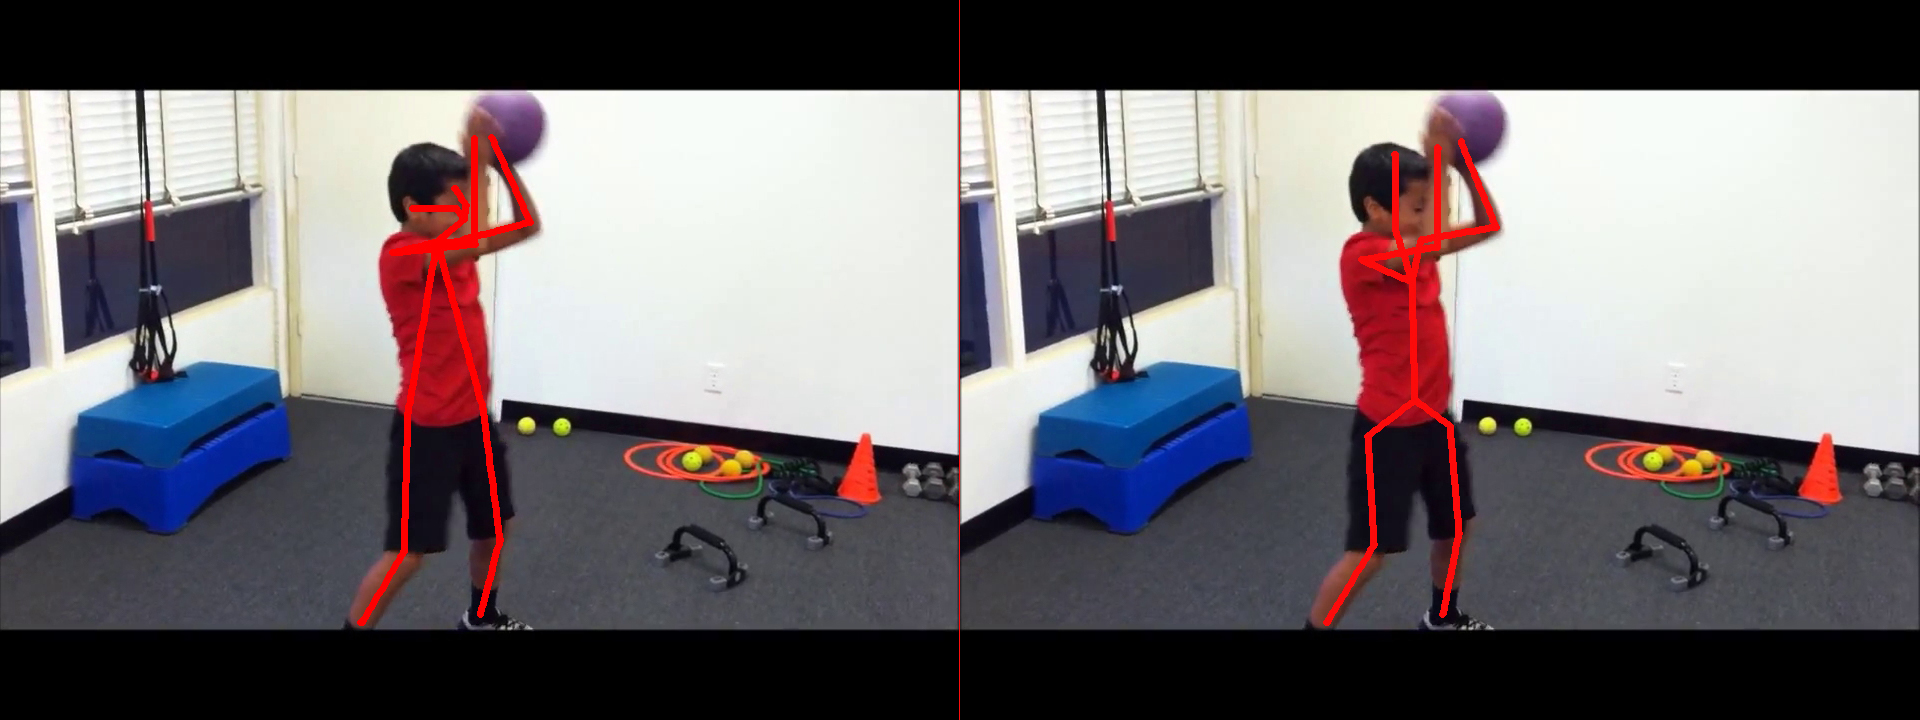
\includegraphics[width=\textwidth]{pic/vs_2.jpg}
	\caption{演示2(左图为COCO标注,右图为MPII标注)}
	\label{vs_2}
\end{figure}

因为本课题是对于人体姿态估计算法的探究,并不需要很多的面部信息标注,且数据点标注信息更多,数据集的照片数量更多,会增加项目的训练时间。因此结合工程实际需要,在后续的实验过程中,本文采用MPII数据集的标注方法,即16个关键节点即可。

\section{基于几何约束的深度回归模块的仿真}

结合第三章中介绍到的深度回归模块,我们进行了训练实验的探究。深度回归模块的仿真是建立在八阶堆叠沙漏网络的基础上的。

\subsection{数据样本}

根据annotions标签文件的包围框信息,对于MPII数据集的图片信息做初步提取,选择出之前八阶堆叠沙漏网络的3000个对象,这样提取出目标对象包围框的数据集,按照256*256的尺寸保存在GPU的内存上,等待深度回归模块的深度信息提取。

\subsection{训练步骤}

为了探究基于几何约束的深度回归模块对于识别精度的提升效果,进行如下实验。

其中骨干网,采用八阶堆叠沙漏网络,预置的参数因子,根据\citing{DBLP:journals/corr/abs-1907-11346}$\gamma$设置为0.71,步骤如下:
首先,骨干网提取输入的人类图像的有用的全局特征。其次,二维图像坐标估计部分从骨干部分获取二维特征图,并使用具有批处理归一化层的三个连续卷积层和ReLU激活函数对其进行上采样。然后,1*1卷积网络被用于产生2D热图,批归一化函数从2D热图提取2D图像坐标$X_R$,$Y_R$。第三部分是深度估计部分。它还从主干部分获取特征映射,并应用全局平均池。然后,合并的特征映射经过1乘1卷积,该卷积输出单个标量值γ。最后的绝对深度值ZR是通过乘以k得到的。

\subsection{训练结果分析}

\begin{table}[]
    \centering
    \begin{tabular}{c|c|c|c|c|c|c|c|c}
        \hline
         网络结构 & Head & Shoulder	& Elbow	& Wrist	& Hip & Knee & Ankle & Mean\\
        \hline
         初始网络 & 73.59 & 70.09 & 61.49 & 58.94 & 60.39 & 49.35 & 50.23 & 60.58\\
        \hline
         网络(深度回归模块) & 64.35 & 62.69 & 57.95 & 54.65 & 58.54 & 48.25 & 49.56 & 56.57\\
        \hline
    \end{tabular}
    \caption{MPII和COCO数据集的MPJPE}
    \label{depth_hg}
\end{table}

由于前两个坐标的识别误差并不大,据\citing{DBLP:journals/corr/abs-1907-11346}关键在于第三个坐标的误差,这个坐标在很大程度上影响整体的识别精度。根据上述结果,我们可以发现,加入深度回归模块以后,对于整个系统算法而言,识别精度得到进一步提高,约4.01mm的提升效果。这验证了设计深度回归模块的正确性以及有效性。因此本文算法最终采取了八阶堆叠沙漏网络以及深度回归模块的设计思路

\section{3D人体姿态估计算法的评价}

在MPII数据集上验证了本文算法。并且可以添加一些自己的测试数据集,以检验识别效果。只要测试数据集的人体骨盆大致位于照片中心,本文算法对一些无标注信息的照片,可以进行人体姿态估计的任务。如图\ref{vs_3}所示

\begin{figure}[h]
	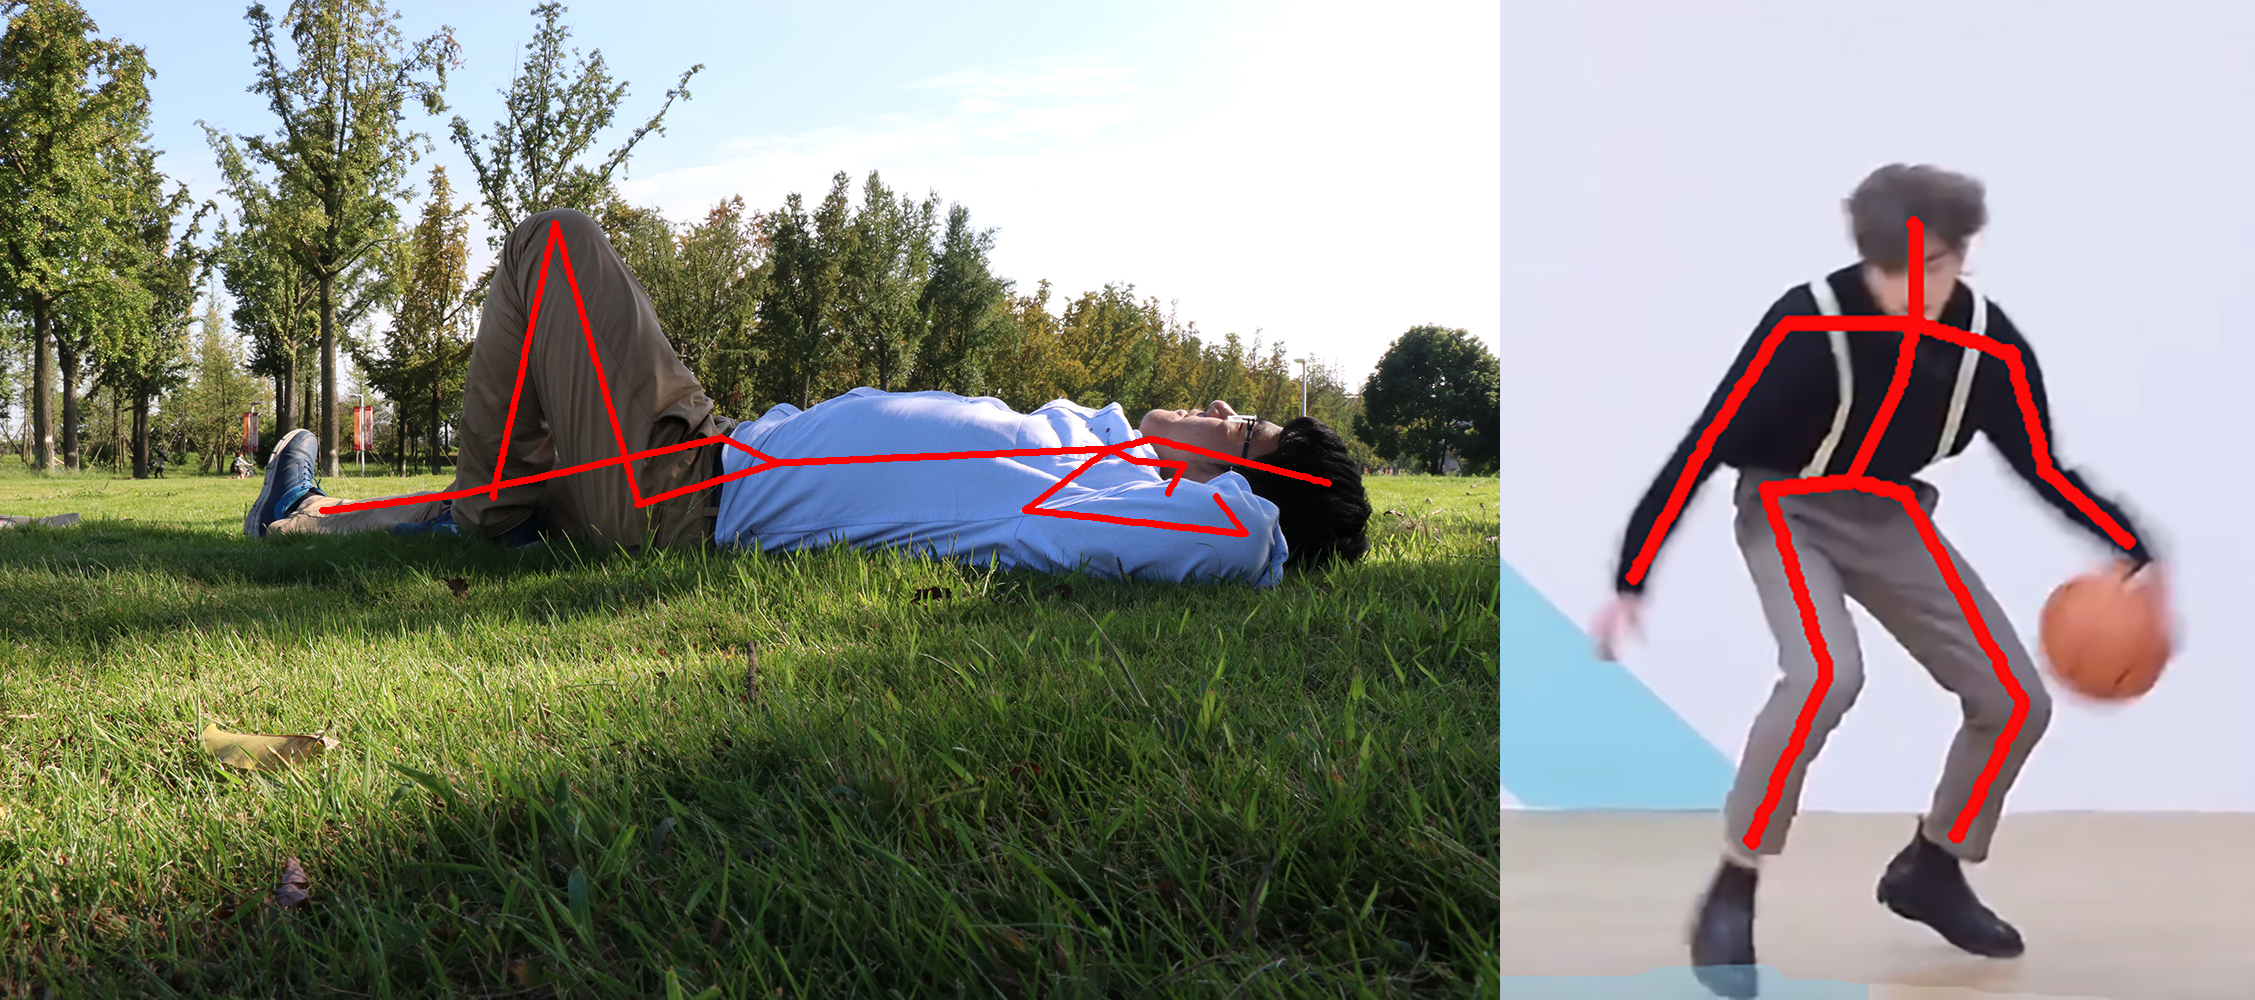
\includegraphics[width=\textwidth]{pic/vs_3.jpg}
	\caption{演示3-无标记照片}
	\label{vs_3}
\end{figure}

结果显示,整个框架算法可以精确地完成多人姿态检测任务。

\begin{figure}[h]
	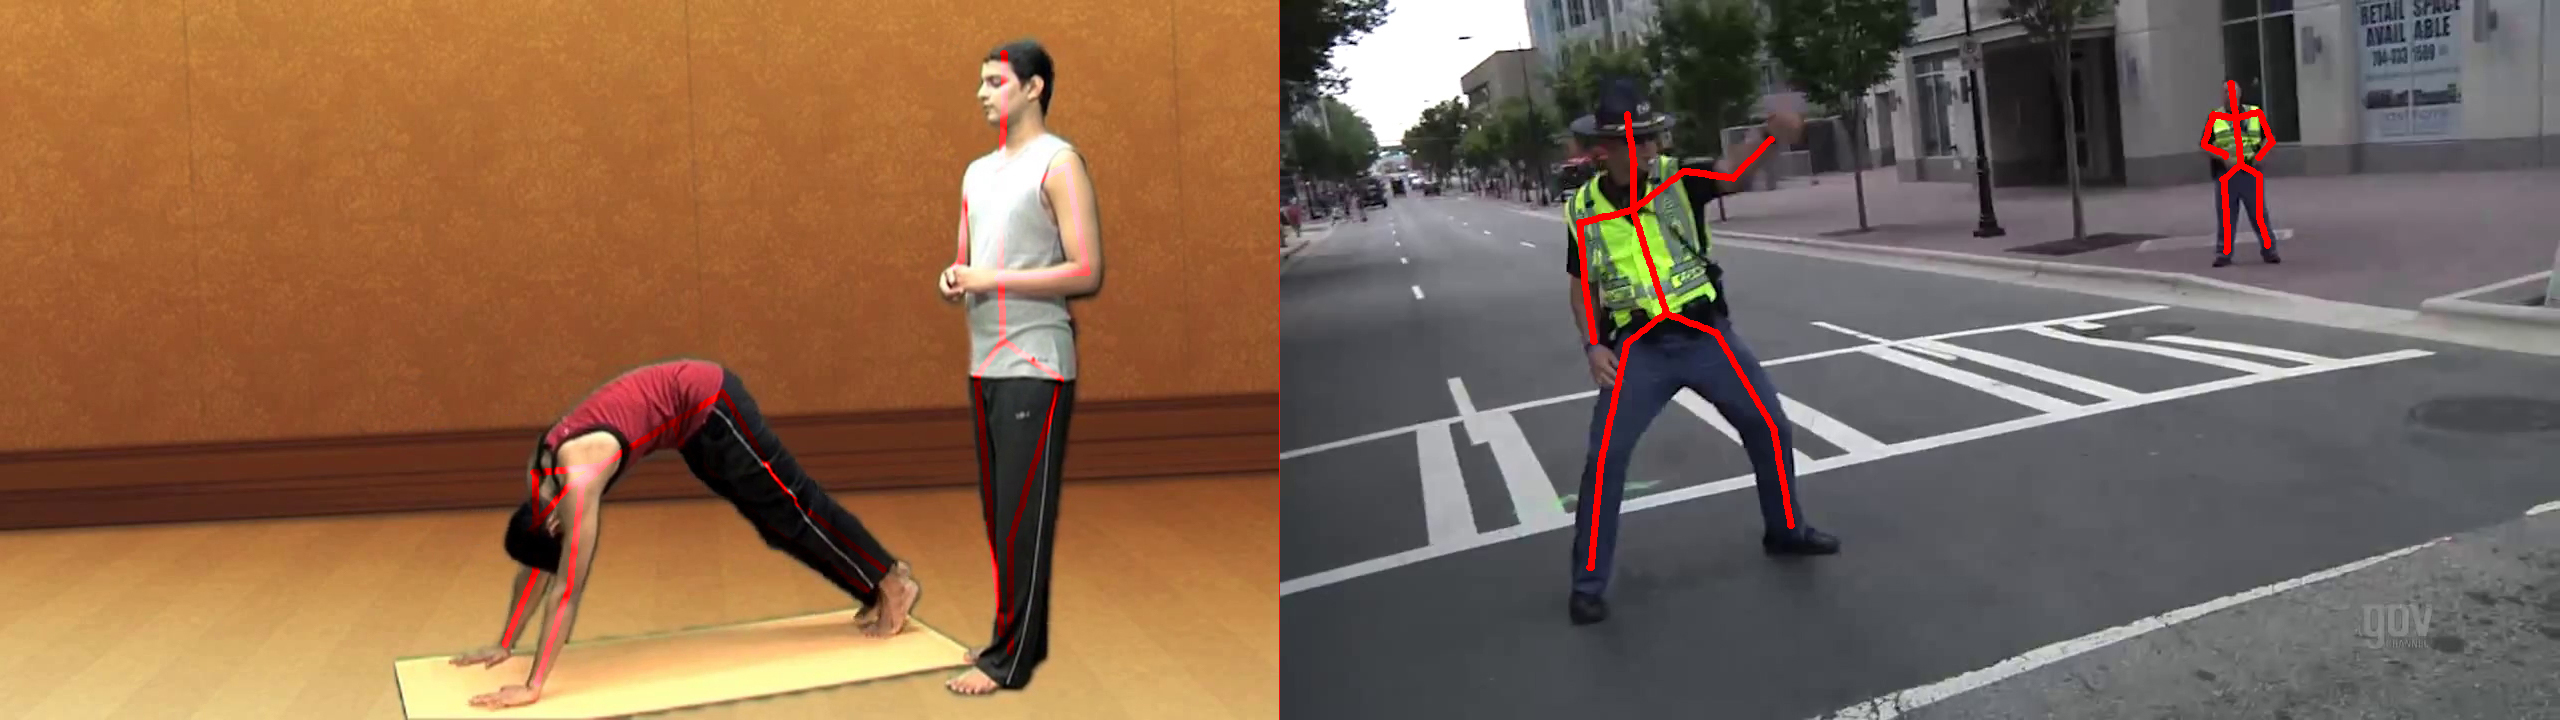
\includegraphics[width=\textwidth]{pic/vs_4.jpg}
	\caption{演示4-多人姿态检测}
	\label{vs_4}
\end{figure}

本文算法虽然在精度上有所改进,但是仍未解决传统计算机视觉中的传统问题,比如因为单目成像造成的视角局限性,导致对于一些特殊情形中的人体姿态估计出现较大误差,甚至出现歧义的情况。就比如存在一些特殊角度,在阻挡的情形下,仍然无法对某些关节点进行判断,或无法进行准确的人体姿态估计。如图\ref{error_1}所示,被测试对象的右肩膀,右肘,右手腕存在很大的误差。

\begin{figure}[h]
	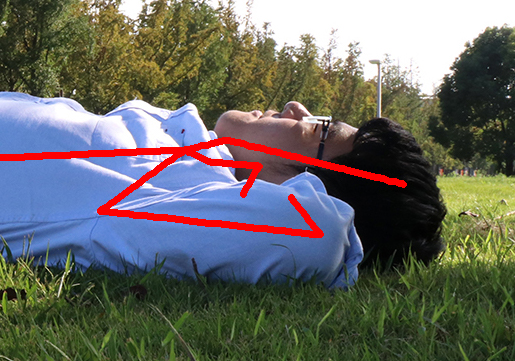
\includegraphics[height=0.6\textwidth]{pic/error_1.jpg}
	\caption{遮挡情况}
	\label{error_1}
\end{figure}

\section{本文的创新点}

1.基于人体骨骼模型,采用树形模型,采用骨盆作为人体中间点,对图像中的人体信息进行语义分割,提取出单人信息,实现多人姿态估计的任务。
2.基于沙漏模块的基础上,设计了八阶堆叠沙漏网络作为训练网络的骨干网络,使得平均关节误差MPJPE优于普通沙漏网络。
3.基于摄像成像原理,结合单孔成像,对人体姿态的第三维坐标进行了几何约束,使得第三维坐标的精确性得到了提高。
4.整体算法框架运行顺利,使得平均关节误差MPJPE达到56mm,满足任务书中的62mm的精度要求。

\section{本章小结}
本章在MPII,COCO数据集上做了实验测试,在比较各阶堆叠沙漏网络的识别效率后,得出了运算效率的最佳堆叠沙漏网络的结构。然后比较了下不同数据集的标注方法对识别效率的影响。最后,对深度回归模块的优化效果进行了验证,确实提高了识别精度。分析了整体算法的优劣,并总结本文的创新点。


